% begin module IVT
\begin{frame}
\begin{theorem}[The Intermediate Value Theorem]
Suppose $f$ is continuous on the closed interval $[a,b]$ and let $N$ be any number between $f(a)$ and $f(b)$, where $f(a) \neq f(b)$.  Then there exists a number $c$ in $(a,b)$ such that $f(c) = N$.
\end{theorem}
\begin{center}
\ \only<handout:0| -1>{%
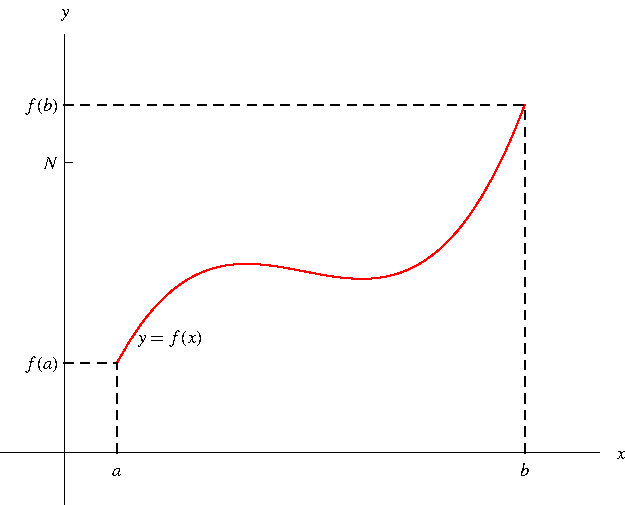
\includegraphics[height=6cm]{continuity/pictures/02-05-ivta.pdf}%
}%
\only<handout:0| 2>{%
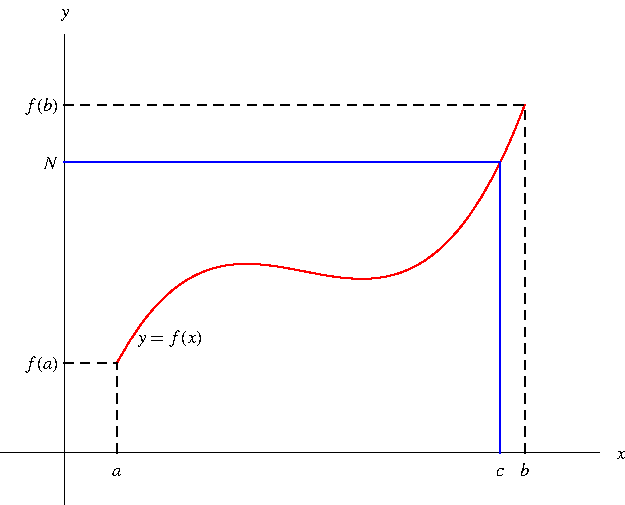
\includegraphics[height=6cm]{continuity/pictures/02-05-ivtb.pdf}%
}%
\only<handout:0| 3>{%
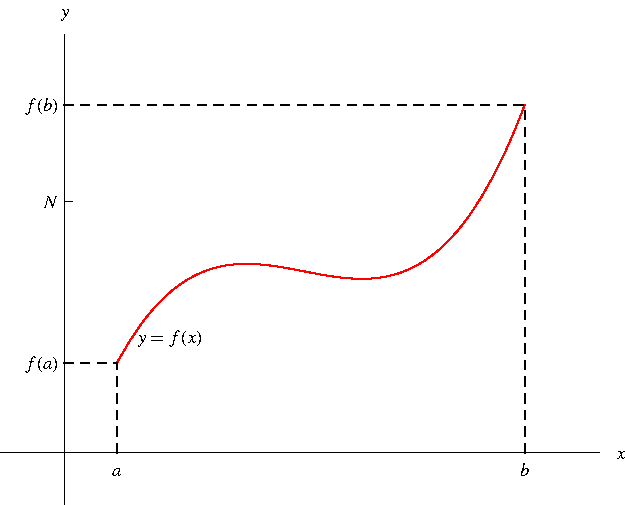
\includegraphics[height=6cm]{continuity/pictures/02-05-ivtc.pdf}%
}%
\only<handout:0| 4>{%
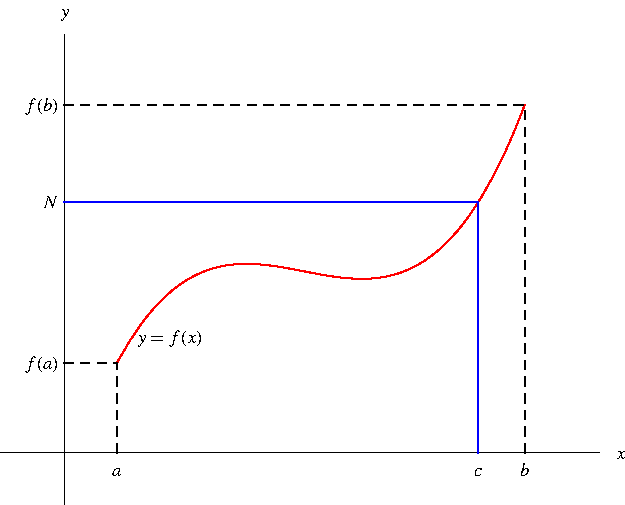
\includegraphics[height=6cm]{continuity/pictures/02-05-ivtd.pdf}%
}%
\only<handout:0| 5>{%
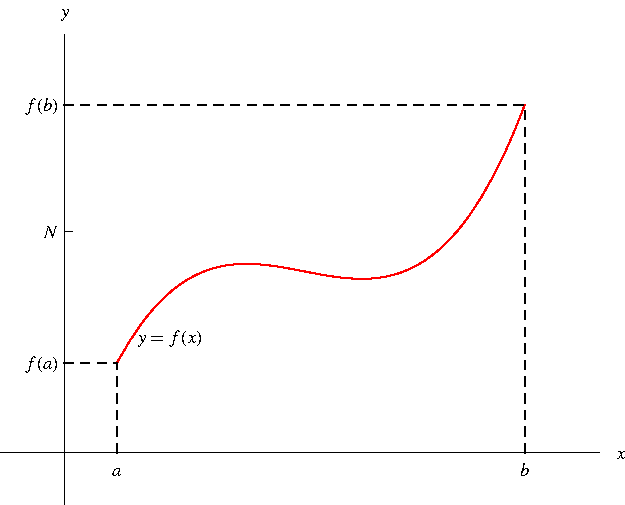
\includegraphics[height=6cm]{continuity/pictures/02-05-ivte.pdf}%
}%
\only<6>{%
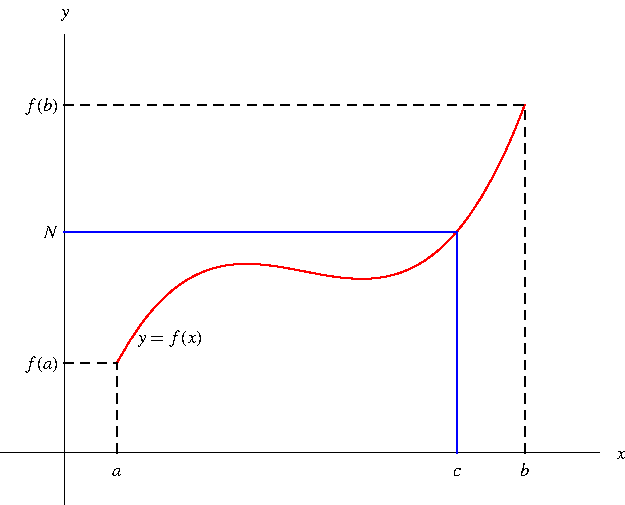
\includegraphics[height=6cm]{continuity/pictures/02-05-ivtf.pdf}%
}%
\only<handout:0| 7>{%
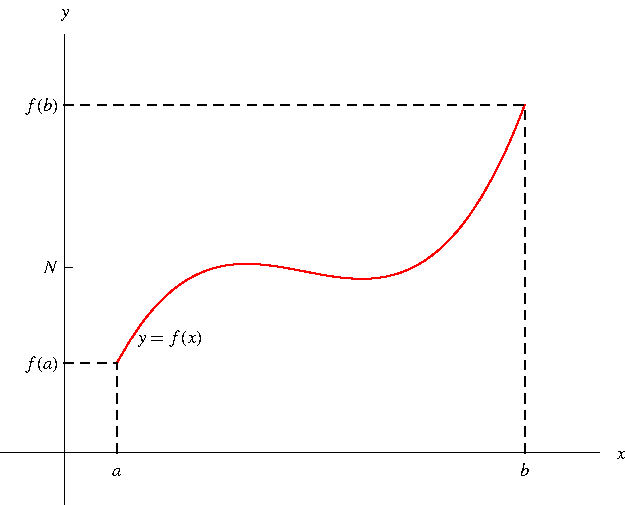
\includegraphics[height=6cm]{continuity/pictures/02-05-ivtg.pdf}%
}%
\only<handout:0| 8->{%
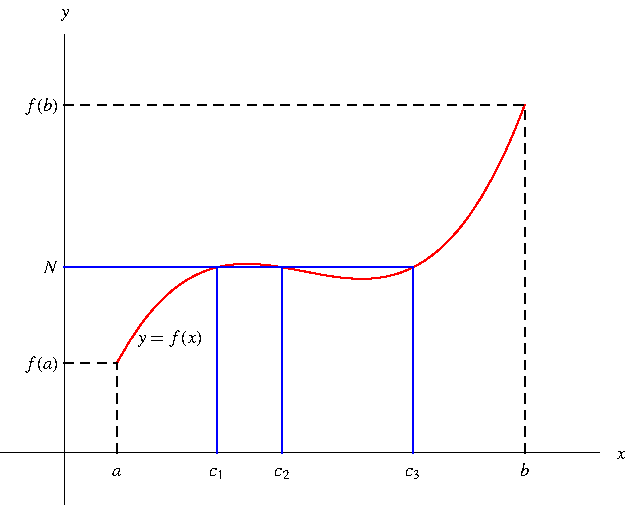
\includegraphics[height=6cm]{continuity/pictures/02-05-ivth.pdf}%
}%
\end{center}
\end{frame}
% end module IVT
